\section{Описание}

Работа в <<ИП>> отличается от метода работы, к которому привыкли в магазинах с формой собственности <<ООО>>
%\raisebox{0pt}[0pt][0pt]{\Large%
%    \textbf{Aaaa\raisebox{-0.3ex}{a}%
%        \raisebox{-0.7ex}{aa}%
%        \raisebox{-1.2ex}{r}%
%        \raisebox{-2.2ex}{g}%
%        \raisebox{-4.5ex}{h}
%    }
%}
Основное это наличие только одного ключа ЕГАИС не зависимо от количества магазинов. Соответственно изменился алгоритм работы с ЕГАИС . Ключ ЕГАИС устанавливается в центральном узле ИП. \textbf{Все действия с алкогольной продукцией производятся только в центральном узле ИП}. Магазины осуществляют только управленческую деятельность. В связи с этим  был принят следующий алгоритм работы ИП с ЕГАИС:
 \begin{itemize}
     \item Получение документа <<Товарно-транспортная накладная ЕГАИС (входящая)>> осуществляется в ЦУ ИП посредством выполнения обмена с ЕГАИС. После получения документа, ответственное лицо заполняет в шапке документа реквизит <<Магазин>>(1), указывая в этом реквизите магазин, для которого предназначен документ, нажимает кнопку \keys{Зарегистрировать документ}(2) для регистрации документа к обмену по нужному магазину. Затем нажимает кнопку \keys{Провести и закрыть}(3)
     Таким образом документ <<Товарно-транспортная накладная ЕГАИС (входящая)>> зарегистрировался по нужному магазину и готов к обмену.

     	\begin{figure}[H]
         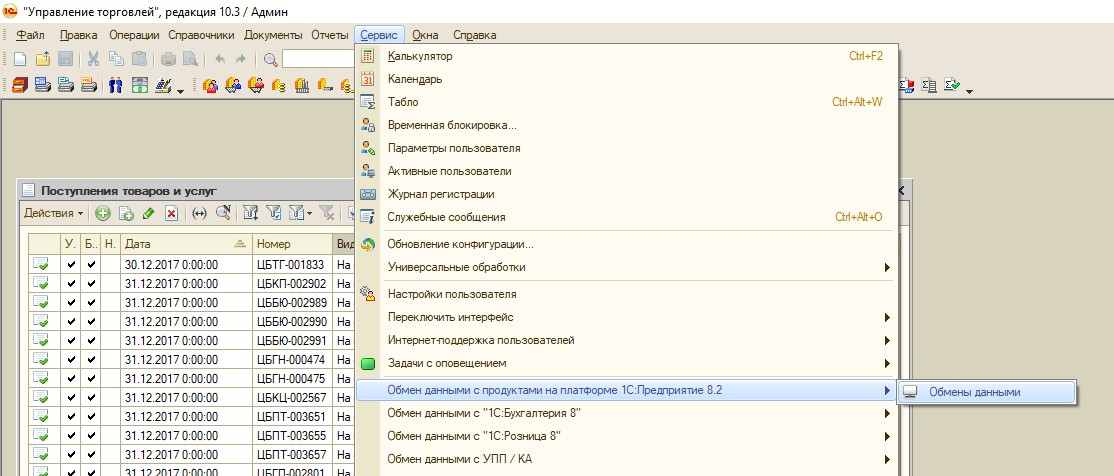
\includegraphics[width=1.0\textwidth]{1.jpg}
         \caption{<<Регистрация документа>>}
         \label{ris:1.jpg}
     \end{figure}


     \item  Ответственное лицо запускает обмен РИБ с указанным магазином и сообщает товароведу данного магазина, о том что им отправлена ТТН.
     \item В магазине ТТН получают. Осуществляют приемку товара \footnote{Так же есть возможность проконтролировать приемку товара по справкам Б}. Заполняют данные о количестве принятого в ТТН (Выполняют проверку алкогольной продукции). Создают <<Поступление товаров>> на основании ТТН, проводят его. Выполняют обмен с ЦУ. Сообщают ответственному лицу о завершении работы с ТТН.
     \item Ответственное лицо выполняя обмен в ЦУ осуществляет прием обработанной ТТН и далее отправляет ТТН в ЕГАИС с соответствующей причиной \footnote{ТТН может быть подтверждена полностью, в случае если весть товар получен и претензий нет. Частично, если часть товара не пришла или товар не качественный или не соответствует накладно. Полный отказ, если товар не пришел, не соответствующего качества или иные причины}.
     \item После подтверждения входящей ТТН, ответственное лицо создает на основании подтвержденной документ <<Передача в регистр №2 ЕГАИС>>  и проводит его. Алкогольная продукция присутствующая в документе перемещается на второй регистр. Ответственный передает данные в ЕГАИС.
     \item В узле магазина  при закрытии кассовой смены создается документ <<Отчет о розничных продажах>>  и с обменом уходит в ЦУ.

     \item В ЦУ на данном этапе в ручном режиме, а в дальнейшем с помощью фонового задания, на основании пришедшего из магазина документа <<Отчет о розничных продажах>>  создается документ  <<Акт списания ЕГАИС>> заполняется списываемой алкогольной продукцией  и отправляется в ЕГАИС. Документ <<Акт списания ЕГАИС>> списывает с остатка алкогольную продукцию в ЕГАИС.
     \item При проведении инвентаризации в магазине, в узле создаются все управленческие документы, в частности <<Списание товаров>> и <<Оприходование товаров>>, котрые после обмена попадают в ЦУ. В ЦУ при наличии в этих документах алкогольной продукции создаются соответственно документы <<Акт списания ЕГАИС>> и <<Акт постановки на баланс ЕГАИС>> осуществляющие движение алкогольной продукции в ЕГАИС.
     \item При возврате товаров поставщику,  вначале создается документ <<Возврат из регистра №2 ЕГАИС>>  в котром указывается конкретная справка Б по которой мы хотим вернуть товар. Алкогольная продукция перемещается на регистр 1. На основании документа <<Возврат товаров поставщику>> создается документ <<Товарно-транспортная накладная ЕГАИС (исходящая)>> и отправляется в ЕГАИС.
      \item При перемещениях товара между магазинами в базе ИП не происходит движения алкоголя по ЕГАИС.

 \end{itemize}
